%% Formatação derivada de reports/compiladores/Relatorio_AOC.tex.
%% Conteúdo técnico validado contra o repositório em 23/09/2026.
\documentclass[
  12pt,
  oneside,
  a4paper,
  english,
  french,
  spanish,
  brazilian,
]{abntex2}

% Pacotes fundamentais preservados do relatório-base.
\usepackage{lmodern}
\usepackage[T1]{fontenc}
\usepackage[utf8]{inputenc}
\usepackage{indentfirst}
\usepackage{color}
\usepackage{graphicx}
\usepackage{microtype}
\usepackage{url}
\usepackage[export]{adjustbox}
\usepackage{multicol}
\usepackage{multirow}
\usepackage{array}
\usepackage{float}
\usepackage{pdflscape}
\usepackage{xcolor}
\usepackage{listings}

\definecolor{verde}{rgb}{0,0.5,0}
\lstdefinelanguage{text}{}
\lstdefinelanguage{assembly}{}
\lstset{
  language=Verilog,
  basicstyle=\ttfamily\tiny,
  keywordstyle=\color{blue},
  stringstyle=\color{verde},
  commentstyle=\color{gray},
  extendedchars=true,
  showspaces=false,
  showstringspaces=false,
  numbers=left,
  numberstyle=\tiny,
  breaklines=true,
  backgroundcolor=\color{green!10},
  breakautoindent=true,
  captionpos=b,
  xleftmargin=0pt,
}

\usepackage[brazilian,hyperpageref]{backref}
\usepackage[alf]{abntex2cite}
\citebrackets()

\renewcommand{\backrefpagesname}{Citado na(s) página(s):~}
\renewcommand{\backref}{}
\renewcommand*{\backrefalt}[4]{%
  \ifcase #1 Nenhuma citação no texto.%
  \or Citado na página #2.%
  \else Citado #1 vezes nas páginas #2.%
  \fi}

\titulo{Plataforma C- e Processador ARM-like:\\Relatório Técnico Inicial para o Laboratório de Sistemas Operacionais}
\autor{Heitor Gabriel Barroso Reis}
\local{São José dos Campos - Brasil}
\data{Setembro de 2026}
\instituicao{
  Universidade Federal de São Paulo - UNIFESP
  \par
  Instituto de Ciência e Tecnologia - Campus São José dos Campos
}
\tipotrabalho{Relatório Técnico}
\preambulo{Relatório inicial que consolida a plataforma de compilação C- e o processador ARM-like existente, estabelece o estado técnico verificado do projeto e registra as lacunas que antecedem o desenvolvimento do Laboratório de Sistemas Operacionais.}

\definecolor{blue}{RGB}{41,5,195}
\makeatletter
\hypersetup{
  pdftitle={\@title},
  pdfauthor={\@author},
  pdfsubject={\imprimirpreambulo},
  pdfcreator={LaTeX with abnTeX2},
  pdfkeywords={abnt}{latex}{abntex2}{processador}{verilog}{fpga}{compiladores}{cminus}{sistemas operacionais},
  colorlinks=true,
  linkcolor=blue,
  citecolor=blue,
  filecolor=magenta,
  urlcolor=blue,
  bookmarksdepth=4,
  hypertexnames=false
}
\makeatother

\setlength{\parindent}{1.3cm}
\setlength{\parskip}{0.2cm}
\makeindex

\begin{document}
\selectlanguage{brazilian}
\frenchspacing

\imprimircapa
\imprimirfolhaderosto*

\setlength{\absparsep}{18pt}
\begin{resumo}
Este relatório estabelece a linha de base técnica para o próximo Laboratório de Sistemas Operacionais. A análise parte de dois trabalhos anteriores: o relatório do processador ARM-like, concluído em 2024, e o relatório de integração do compilador C-, concluído em 2025. Como o hardware foi modificado depois dessas entregas, as descrições históricas foram confrontadas com o RTL, o projeto Quartus, o compilador, o montador e o simulador presentes no repositório em setembro de 2026. O documento consolida somente informações confirmadas, descreve a interface entre código C-, código de máquina e FPGA e identifica divergências relevantes em memória, inicialização, temporização, desvios e diagramas. O Sistema Operacional ainda não existe; por isso, escalonamento, processos, chamadas de sistema, memória virtual e sistema de arquivos são apresentados apenas como lacunas futuras, sem alegação de implementação.

\noindent
\textbf{Palavras-chaves}: Processador. Verilog. FPGA. Compiladores. C-. Arquitetura ARM-like. Sistemas Operacionais. Linha de base.
\end{resumo}

\pdfbookmark[0]{\listfigurename}{lof}
\listoffigures*
\clearpage
\pdfbookmark[0]{\listtablename}{lot}
\listoftables*
\clearpage
\pdfbookmark[0]{\contentsname}{toc}
\tableofcontents*

\textual

\chapter{Introdução}
\label{cap:introducao}

O projeto reúne duas camadas que precisam concordar: um processador didático descrito em Verilog e uma cadeia de compilação que traduz programas C- para a linguagem de máquina desse processador. O relatório de Arquitetura e Organização de Computadores documentou a primeira versão integrada do hardware, enquanto o relatório de Compiladores passou a documentar também o front-end, a representação intermediária, o back-end e o montador. Ambos preservam decisões importantes, mas nenhum relatório histórico, isoladamente, constitui a especificação da versão atual.

Este documento tem três funções. A primeira é registrar a fundamentação que continua válida: organização Harvard, orientação RISC, instruções fixas de 32 bits, banco de registradores, execução condicional e separação entre front-end e back-end \cite{patterson2017,compOrgDes,compiladoresLouden}. A segunda é descrever a implementação observável no repositório. A terceira é identificar o que falta antes de iniciar um Sistema Operacional, sem antecipar funcionalidades que ainda não foram projetadas ou implementadas.

\section{Objetivo}

O objetivo é oferecer uma base única e rastreável para o próximo laboratório. A consolidação não é uma simples união textual: uma afirmação antiga só é mantida quando concorda com as fontes atuais. Quando há conflito, registra-se o comportamento atual e a divergência. Quando não existe evidência suficiente, a lacuna permanece explícita.

\section{Método e fontes de verdade}

A auditoria adotou a seguinte precedência:
\begin{enumerate}
  \item RTL e configuração Quartus em \texttt{processor/Processor/};
  \item compilador, montador e simulador em \texttt{compiler/} e \texttt{tools/};
  \item testes executáveis e artefatos reproduzíveis;
  \item documentação corrente;
  \item relatórios e imagens anteriores, usados como contexto histórico.
\end{enumerate}

As fontes documentais comparadas foram:
\begin{itemize}
  \item relatório histórico do processador: \path{reports/processador/processadorARM_2024_2.pdf};
  \item complemento técnico de codificação, localizado em \path{reports/processador/};
  \item relatório-base de compiladores e de formatação: \path{Relatorio_AOC.tex}, localizado em \path{reports/compiladores/}.
\end{itemize}
A matriz detalhada de rastreabilidade acompanha este projeto em \texttt{COMPARACAO.md}.

\chapter{Fundamentação preservada}
\label{cap:fundamentacao}

\section{Organização Harvard e orientação RISC}

A separação entre memória de instruções e memória de dados caracteriza uma organização Harvard. No projeto atual, a ROM é endereçada pelo contador de programa, enquanto a RAM recebe endereços e dados do caminho de execução. Essa separação permanece coerente com os relatórios anteriores e com o RTL \cite{compOrgDes,compArchi}.

O processador é ARM-like, e não uma implementação binariamente compatível com ARM. A inspiração aparece na largura fixa das instruções, no campo de condição, no registrador de estado e em operações de branch com link. A codificação, a quantidade de flags e a semântica de memória são próprias do projeto \cite{ARMtechnical}.

A \autoref{fig:harvard-von-neumann} resume a diferença conceitual que fundamenta a organização adotada. Ela não representa as conexões internas do processador; apenas evidencia que, em Harvard, programa e dados ocupam memórias distintas. No projeto, essa separação se concretiza nos módulos \texttt{InstructionMemory} e \texttt{DataMemory}.

\begin{figure}[H]
  \centering
  \caption{Comparação conceitual entre organizações Harvard e von Neumann}
  \label{fig:harvard-von-neumann}
  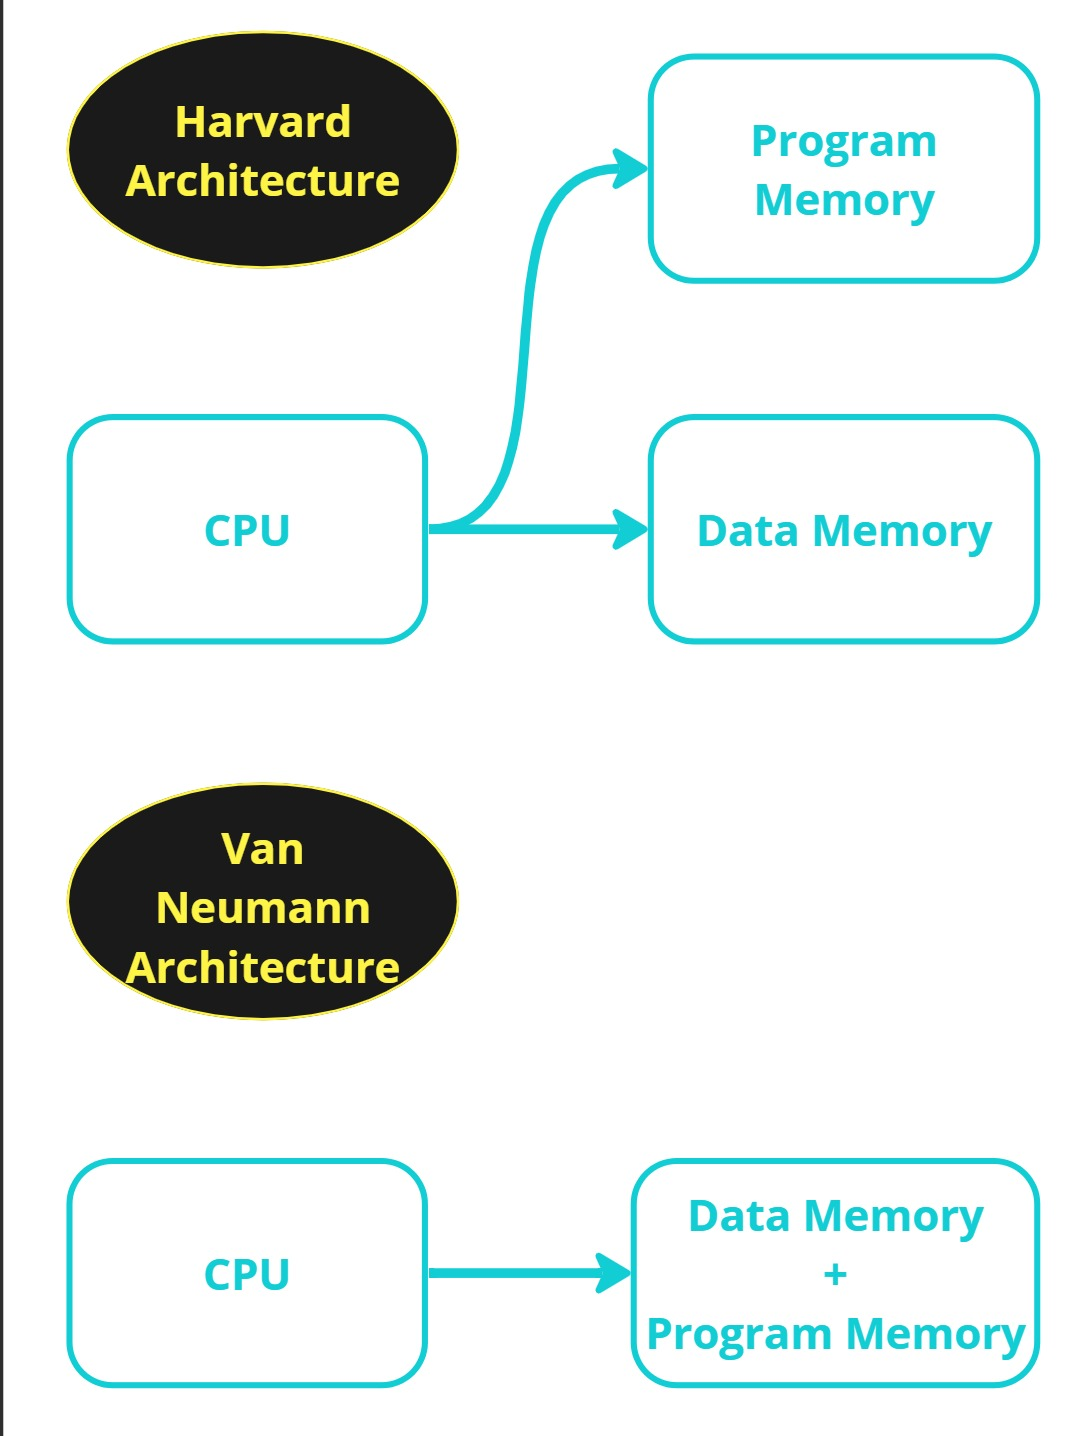
\includegraphics[height=0.62\textheight]{figuras/harvard-vs-von-neumann.jpg}
  \legend{Fonte: acervo do relatório de compiladores. Figura conceitual validada contra a separação de memórias do RTL atual.}
\end{figure}

\section{Compilação como contrato entre software e hardware}

O compilador transforma C- em uma AST, valida o programa, produz IR textual, gera assembly e codifica palavras de 32 bits. A saída só é correta quando montador, simulador e RTL interpretam os mesmos campos. Portanto, a ISA é uma interface compartilhada e qualquer alteração nela exige validação coordenada.

A \autoref{fig:fluxo-compilacao} organiza esse contrato como uma sequência ponta a ponta. A figura foi preservada do relatório de compiladores porque suas etapas continuam presentes no repositório atual. Os nomes das raias representam responsabilidades lógicas: no front-end, várias delas cooperam dentro do mesmo executável em C; no back-end, alocação, geração de assembly e parte do gerenciamento de símbolos estão reunidos em módulos Python. Assim, o diagrama descreve o fluxo de informação, e não processos independentes.

\begin{landscape}
\begin{figure}[p]
  \centering
  \caption{Fluxo integrado de C- até o código binário do processador}
  \label{fig:fluxo-compilacao}
  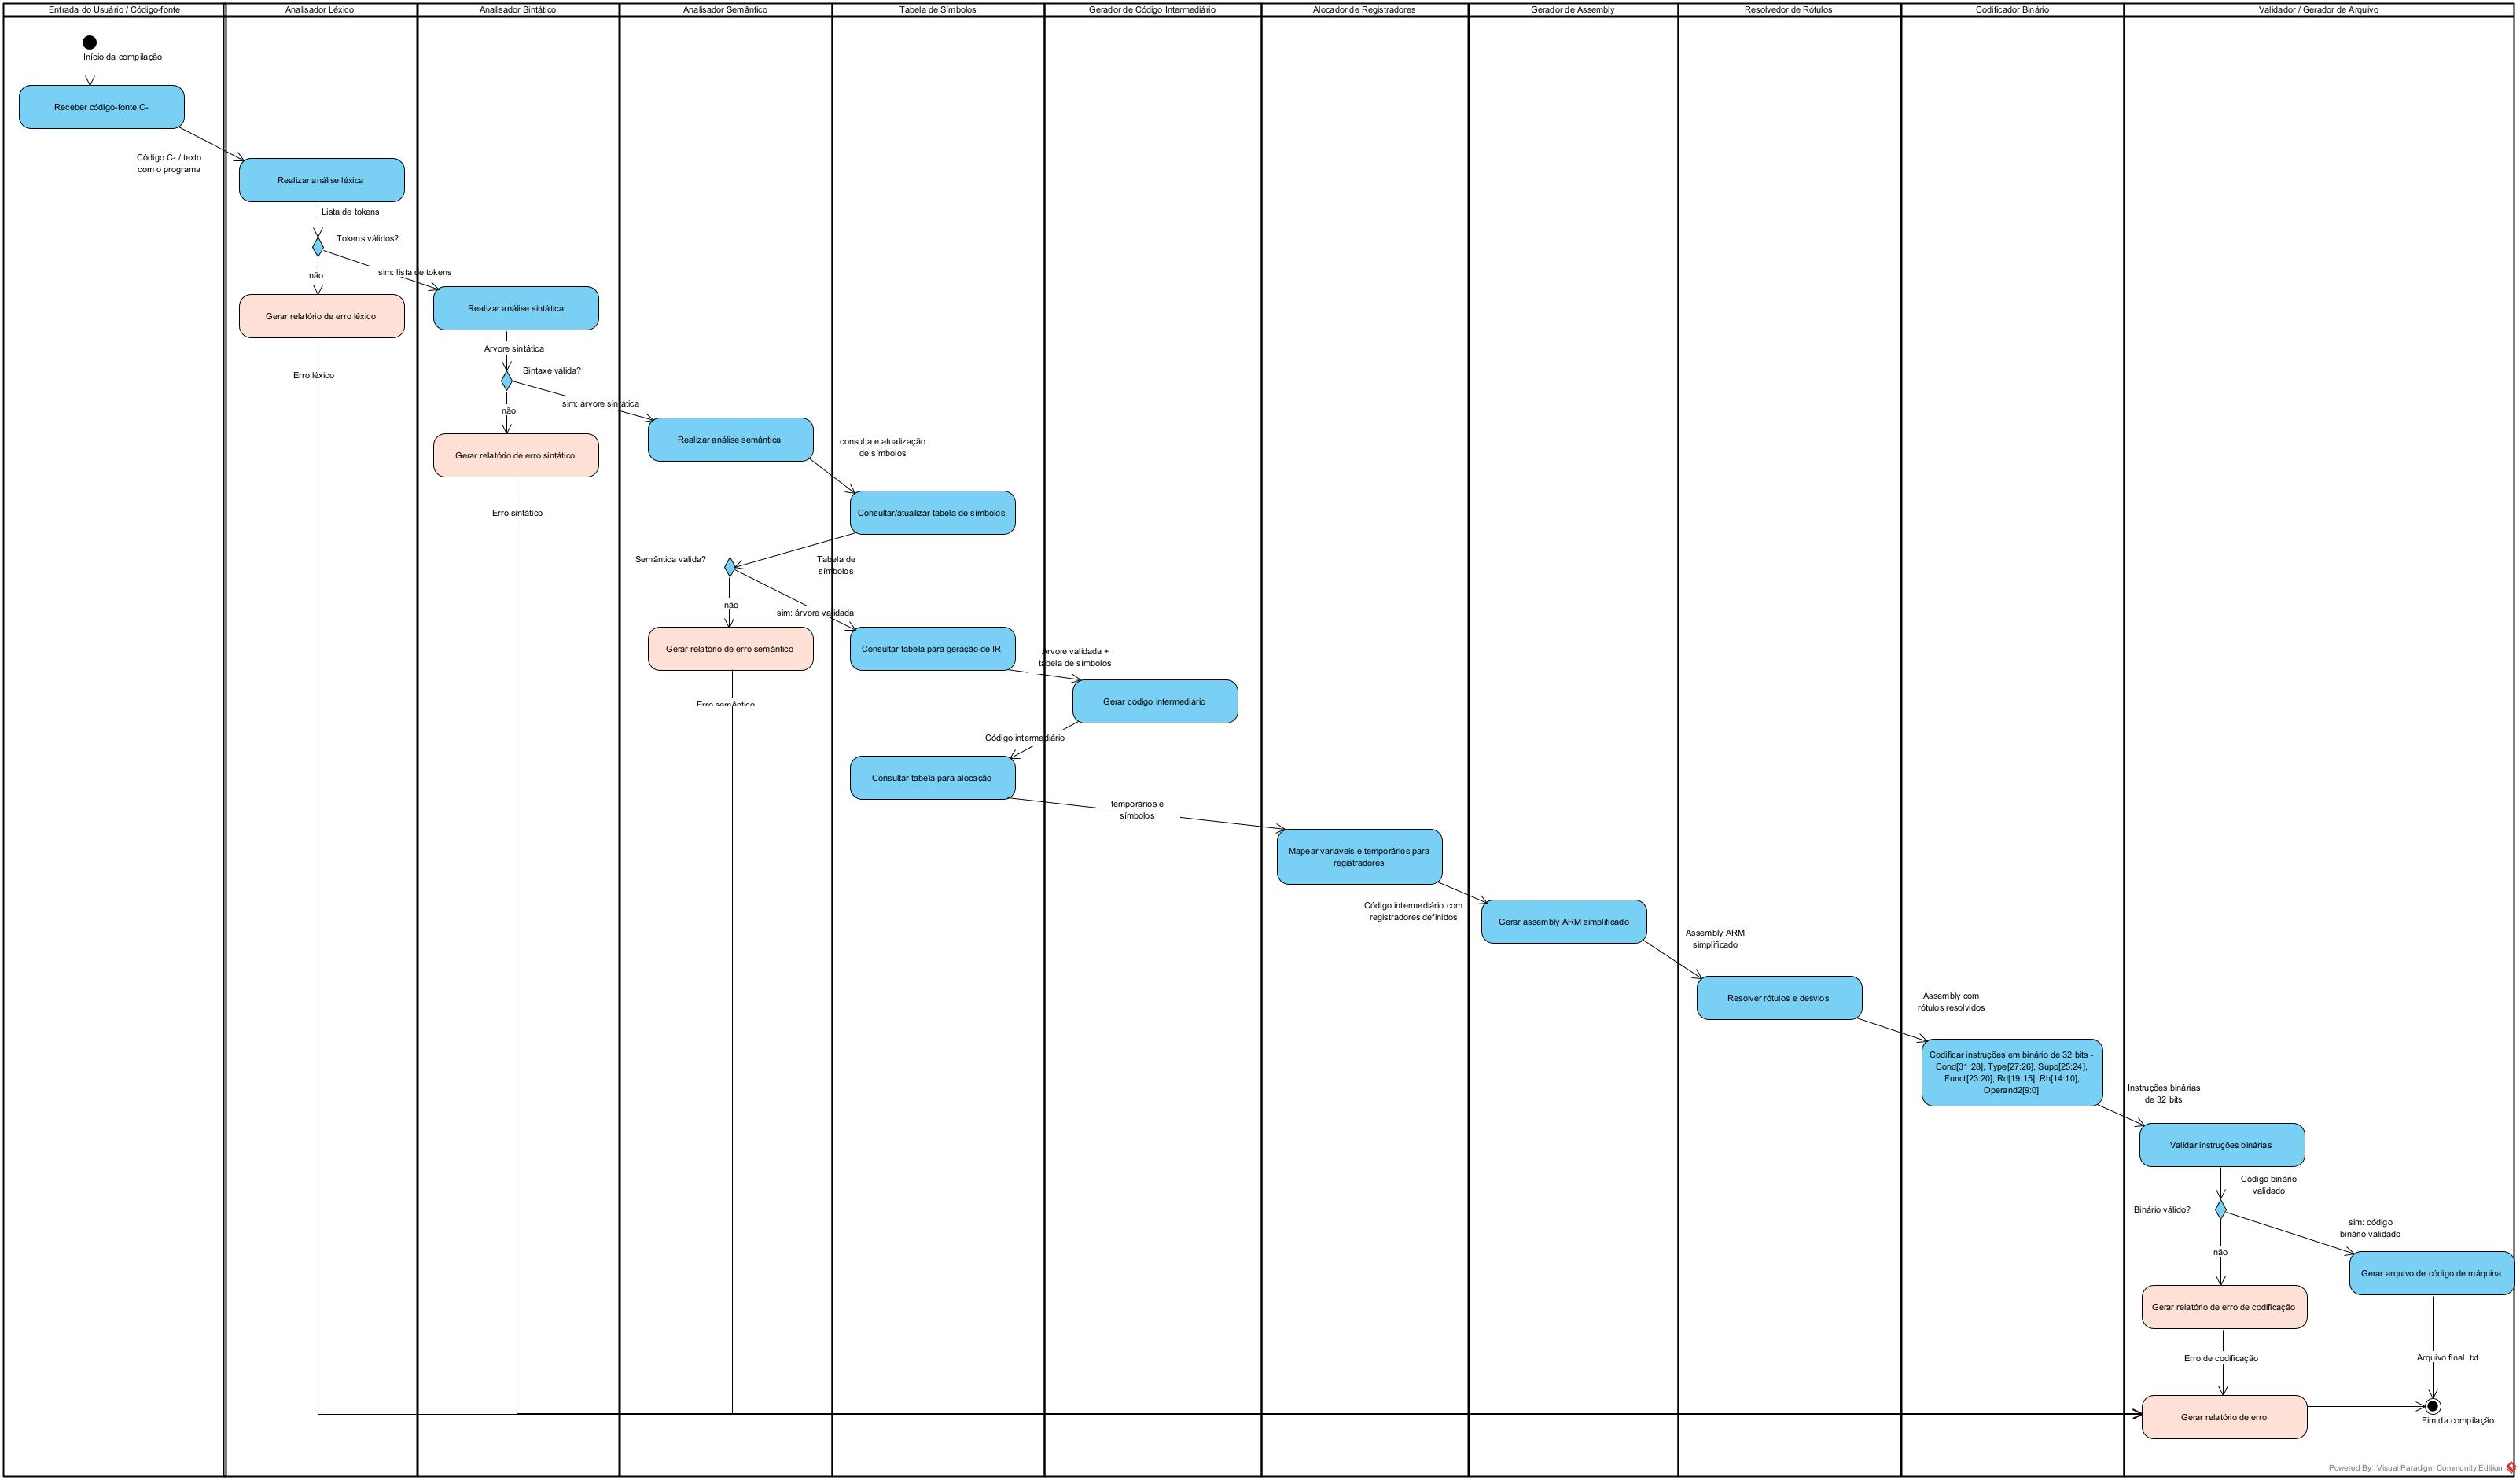
\includegraphics[width=0.96\linewidth]{figuras/fluxo-compilacao-cminus.jpg}
  \legend{Fonte: relatório de compiladores, validado contra \texttt{compiler/main.c}, \texttt{compiler/src/}, \texttt{compiler/codegen/} e \texttt{tools/run\_machine\_code.py}.}
\end{figure}
\end{landscape}

\chapter{Estado atual do processador}
\label{cap:processador}

\section{Projeto FPGA e interface externa}

O projeto Quartus seleciona a família Cyclone IV E, o dispositivo \texttt{EP4CE115F29C7} e a entidade de topo \texttt{Processor}. A pinagem corresponde ao kit DE2-115 \cite{DE2-115}. O módulo de topo recebe \texttt{CLOCK\_50}, chaves e botões; expõe oito displays de sete segmentos, um LED, o último valor de saída e o PC.

\begin{figure}[H]
  \centering
  \caption{Kit FPGA DE2-115 utilizado pelo projeto}
  \label{fig:de2-115}
  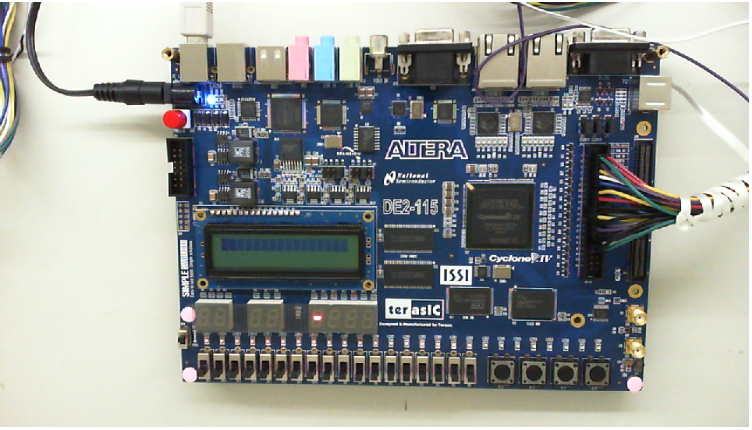
\includegraphics[width=0.72\textwidth]{figuras/de2-115.png}
  \legend{Fonte: acervo do relatório anterior, arquivo \texttt{reports/compiladores/Imagens/FPGA.png}.}
\end{figure}

\begin{table}[H]
\centering
\ABNTEXfontereduzida
\caption{Interface externa confirmada no módulo \texttt{Processor}}
\label{tab:interface}
\begin{tabular}{|p{0.23\textwidth}|p{0.62\textwidth}|}
\hline
\textbf{Sinal} & \textbf{Função observada} \\
\hline
\texttt{SW[17]} & Bloqueia o clock efetivo quando está em nível alto. \\
\hline
\texttt{SW[16]} & Reinicia o PC e o detector associado à entrada; outros bancos não possuem reset explícito no RTL atual. \\
\hline
\texttt{SW[15]} & Confirma a instrução \texttt{in}; a espera termina em uma transição de descida. \\
\hline
\texttt{SW[7:0]} & Valor periférico, estendido para 32 bits na conexão de topo. \\
\hline
\texttt{LEDR[0]} & Resultado da verificação da condição da instrução. \\
\hline
\texttt{HEX6--HEX7} & Dois dígitos decimais menos significativos do último valor de \texttt{out}. \\
\hline
\texttt{HEX0--HEX3} & Representação decimal do endereço corrente de instrução. \\
\hline
\end{tabular}
\legend{Fonte: O autor, com base em \texttt{Processor.v}, \texttt{output\_module.v} e \texttt{Processor.qsf}.}
\end{table}

\section{Formato da instrução}

O formato confirmado possui 32 bits e é compartilhado pelo montador e pelo decodificador do RTL.

\begin{table}[H]
\centering
\ABNTEXfontereduzida
\caption{Campos atuais da instrução}
\label{tab:campos}
\begin{tabular}{|p{0.17\textwidth}|p{0.16\textwidth}|p{0.52\textwidth}|}
\hline
\textbf{Campo} & \textbf{Bits} & \textbf{Semântica} \\
\hline
\texttt{Cond} & \texttt{31:28} & Condição verificada contra Z e N. \\
\hline
\texttt{Type} & \texttt{27:26} & \texttt{00}: dados; \texttt{01}: memória; \texttt{11}: branch; \texttt{10}: não utilizado. \\
\hline
\texttt{Supp} & \texttt{25:24} & Bit 25 seleciona imediato; bit 24 solicita atualização do CPSR. \\
\hline
\texttt{Funct} & \texttt{23:20} & Operação; em branches, os bits 23 e 22 controlam link e retorno. \\
\hline
\texttt{Rd} & \texttt{19:15} & Registrador geral de destino. \\
\hline
\texttt{Rh} & \texttt{14:10} & Primeiro operando ou dado de store. \\
\hline
\texttt{Operand2} & \texttt{9:0} & Imediato com sinal ou \texttt{Ro} em \texttt{9:5}, com zeros em \texttt{4:0}. \\
\hline
\end{tabular}
\legend{Fonte: O autor, com base em \texttt{ControlUnit.v}, \texttt{assembler.py} e \texttt{run\_machine\_code.py}.}
\end{table}

\begin{table}[H]
\centering
\ABNTEXfontereduzida
\caption{Operações aceitas pelo montador e modeladas no processador}
\label{tab:operacoes}
\begin{tabular}{|p{0.22\textwidth}|p{0.62\textwidth}|}
\hline
\textbf{Classe} & \textbf{Operações} \\
\hline
Dados & \texttt{add}, \texttt{sub}, \texttt{mul}, \texttt{div}, \texttt{and}, \texttt{or}, \texttt{xor}, \texttt{not}, \texttt{mov}, \texttt{in}, \texttt{out}. \\
\hline
Memória & \texttt{load} e \texttt{store}, com endereço fornecido por registrador no fluxo gerado. \\
\hline
Controle & \texttt{b}, \texttt{bl} e o retorno codificado pelo montador como branch para o link dedicado. \\
\hline
\end{tabular}
\legend{Fonte: O autor.}
\end{table}

As condições implementadas são \texttt{do}, \texttt{eq}, \texttt{neq}, \texttt{gt}, \texttt{gteq}, \texttt{lt} e \texttt{lteq}. Apenas Z e N são produzidas; C e V permanecem zeradas. A condição histórica \texttt{NOT} não é aceita pelo montador e cai no caso falso do \texttt{FlagVerifier}; por isso, não integra a ISA atual.

\subsection{Semântica da ULA e flags}

A ULA recebe \texttt{RhValue} como primeiro operando e seleciona entre \texttt{RoValue} e o imediato estendido para o segundo. Para operações de dados, os opcodes \texttt{0000--0110} implementam adição, subtração, multiplicação, divisão, AND, OR e XOR. O opcode \texttt{0111}, embora exposto pelo montador com o mnemônico \texttt{not}, executa \texttt{-A} em \texttt{alu.v}; portanto, sua semântica atual é negação aritmética, não complemento bit a bit. \texttt{MOV}, \texttt{IN} e \texttt{OUT} ocupam \texttt{1000}, \texttt{1001} e \texttt{1010}.

A \autoref{fig:ula-waveform} é uma captura arquivada cuja sequência foi conferida contra essa lógica combinacional. Ela mostra, para \texttt{RhValue=2} e \texttt{RoValue=8}, resultados 10, $-6$, 16 e 0 para ADD, SUB, MUL e DIV, seguidos por $-2$ no opcode \texttt{0111} e 2 em MOV. A figura é evidência ilustrativa compatível, mas não substitui um testbench autochecking atual nem demonstra fechamento de timing.

\begin{figure}[H]
  \centering
  \caption{Captura arquivada da ULA para diferentes opcodes e flags Z/N}
  \label{fig:ula-waveform}
  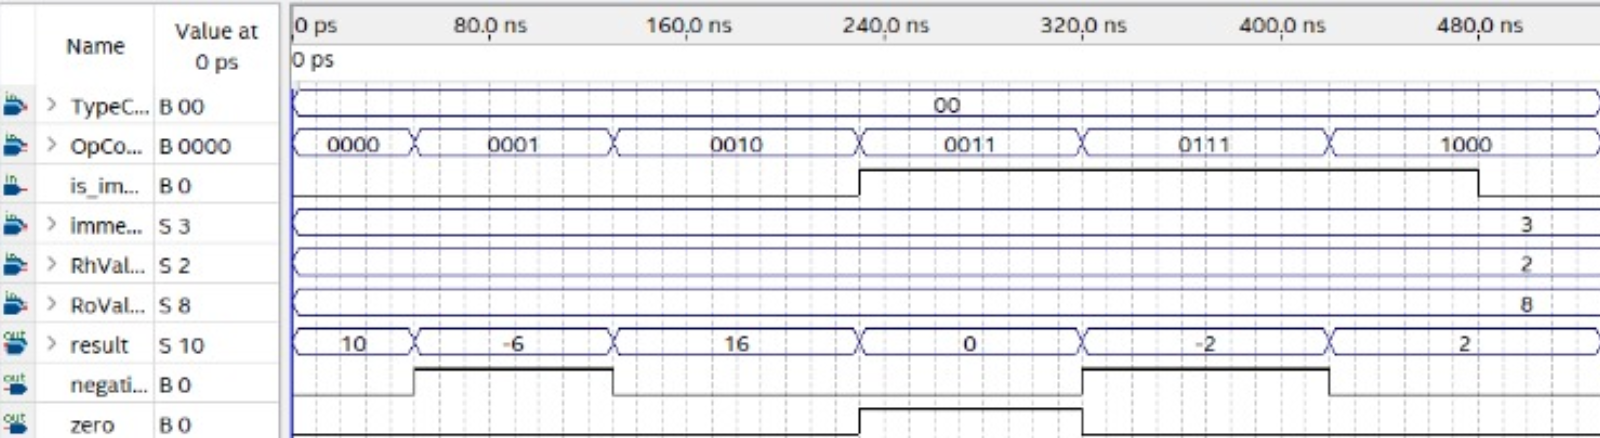
\includegraphics[width=\textwidth]{figuras/ula-control-waveform.png}
  \legend{Fonte: acervo do relatório de compiladores, conferido contra \texttt{ALUControl.v} e \texttt{alu.v}.}
\end{figure}

\section{Caminho de dados verificado}

O caminho de dados ativo foi reconstruído a partir de \texttt{integrated.v}. A instrução sai da ROM e é particionada pela unidade de controle. O banco fornece \texttt{RhValue}, \texttt{RoValue} e o link dedicado. O controlador da ULA escolhe entre \texttt{RoValue} e o imediato estendido; a ULA executa a operação ou encaminha o operando necessário a memória e branch. O multiplexador de escrita escolhe o resultado da ULA ou a saída da RAM. A condição, combinada com o tipo da instrução, habilita escritas no banco, no link, na RAM e a atualização do PC.

Não há, no acervo atual, uma figura validada desse caminho. O diagrama histórico foi rejeitado porque representa incremento de PC por quatro, endereço de RAM oriundo da ULA e campos de instrução incompatíveis com o RTL atual. Até que seja produzido um novo diagrama diretamente da implementação, esta descrição textual e as conexões em \texttt{integrated.v} são a referência.

\section{Registradores, flags e controle de fluxo}

O banco contém 32 registradores gerais de 32 bits e um registrador de link dedicado. Escritas ocorrem na borda positiva do clock efetivo; leituras são registradas na borda positiva de \texttt{fast\_clock}. O sinal de reset existe na interface do banco, mas não é utilizado internamente, de modo que não se deve afirmar que todos os registradores são zerados no reset.

O PC é atualizado na borda negativa do clock. Se a condição falha, ele avança uma palavra. Se a condição passa, um branch imediato soma ao PC um deslocamento com sinal; um branch por registrador usa diretamente \texttt{RoValue}; e a forma de retorno usa o link dedicado. \texttt{bl} salva \texttt{PC+1} na borda positiva antes da atualização do PC.

\begin{table}[H]
\centering
\ABNTEXfontereduzida
\caption{Semântica atual de branch}
\label{tab:branch}
\begin{tabular}{|p{0.25\textwidth}|p{0.57\textwidth}|}
\hline
\textbf{Forma} & \textbf{Efeito quando a condição é verdadeira} \\
\hline
Imediata & \texttt{PC := PC + signExtend(imm10)}. \\
\hline
Por registrador & \texttt{PC := RoValue}. \\
\hline
Branch-and-link & \texttt{Link := PC+1}, seguido do destino imediato ou por registrador. \\
\hline
Retorno dedicado & \texttt{PC := LinkValue}. \\
\hline
\end{tabular}
\legend{Fonte: O autor, com base em \texttt{ControlUnit.v}, \texttt{registerBank.v} e \texttt{PC\_main.v}.}
\end{table}

\section{Memórias e temporização}

A ROM é uma matriz de 1024 palavras de 32 bits, endereçada pelos dez bits menos significativos do PC e inicializada no fluxo Quartus por \texttt{modules/program.mif}. O arquivo ativo pode ser trocado pelos alvos de Make que selecionam \texttt{program1.mif} a \texttt{program10.mif}. A descrição antiga baseada em arquivo \texttt{.txt} não corresponde à versão atual.

A RAM tem profundidade de 64 endereços. Há, contudo, uma inconsistência estrutural importante: \texttt{DataMemory.v} declara largura padrão de 64 bits, enquanto ULA, banco, compilador e simulador usam palavras de 32 bits. As conexões truncam ou estendem valores implicitamente. Portanto, este relatório não normaliza a RAM como ``64 palavras de 32 bits''; registra a intenção de 32 bits e a declaração RTL atual de 64 bits como uma pendência de correção e validação.

Também não existe hoje uma separação física comprovada entre pilha e dados globais. O back-end reserva conceitualmente 64 palavras para a pilha e inicia os globais no endereço 64, mas o RTL usa somente seis bits de endereço e o simulador aplica máscara de 64 posições. Assim, o endereço 64 volta à posição zero. Os testes atuais podem passar quando os intervalos efetivamente usados não colidem, mas isso não constitui isolamento de regiões. O mapa de memória precisa ser redefinido antes de sustentar processos, pilhas múltiplas ou proteção.

O projeto usa pulsos derivados de \texttt{CLOCK\_50}: um clock efetivo mais lento e um \texttt{fast\_clock}. Há lógica acionada por bordas desses dois sinais e não existe arquivo SDC no conjunto atual. Essa arquitetura requer revisão de temporização e CDC antes que o hardware seja usado como base confiável para mecanismos de SO.

\chapter{Estado atual do compilador}
\label{cap:compilador}

O compilador é uma cadeia de dois programas coordenados por arquivos intermediários. O executável C realiza análise léxica, sintática e semântica, mantém a AST e a tabela de símbolos e só emite IR quando o programa é válido. Em seguida, o back-end Python consome essa IR, constrói sua visão de símbolos e memória, gera assembly e chama o montador. O produto final é uma sequência de palavras de 32 bits que pode alimentar o simulador de máquina e o gerador de MIF.

\section{Arquitetura dos módulos}

A \autoref{fig:hierarquia-compilador} complementa a visão sequencial com os arquivos e estruturas concretos da implementação. No front-end, \texttt{main.c} coordena o lexer e o parser; as ações da gramática constroem nós de \texttt{syntax\_tree}, registram declarações e manipulam a pilha de escopos. \texttt{semantic.c} percorre a AST com apoio da tabela de símbolos, enquanto \texttt{ir.c} emite a representação intermediária. No back-end, \texttt{codegen.py} reúne o gerenciador de dados, o alocador de registradores e o contexto de funções; \texttt{assembler.py} estabiliza o layout, resolve rótulos e codifica as instruções.

O diagrama também evidencia duas tabelas de símbolos distintas. A estrutura em C registra declarações, tipos, escopos, linhas de uso e assinaturas durante a análise. A estrutura em Python é reconstruída a partir da IR para apoiar endereços, tipos e geração de código. Elas cooperam por meio do contrato textual da IR, mas não compartilham memória durante a execução.

\begin{landscape}
\begin{figure}[p]
  \centering
  \caption{Hierarquia dos módulos do compilador e suas relações atuais}
  \label{fig:hierarquia-compilador}
  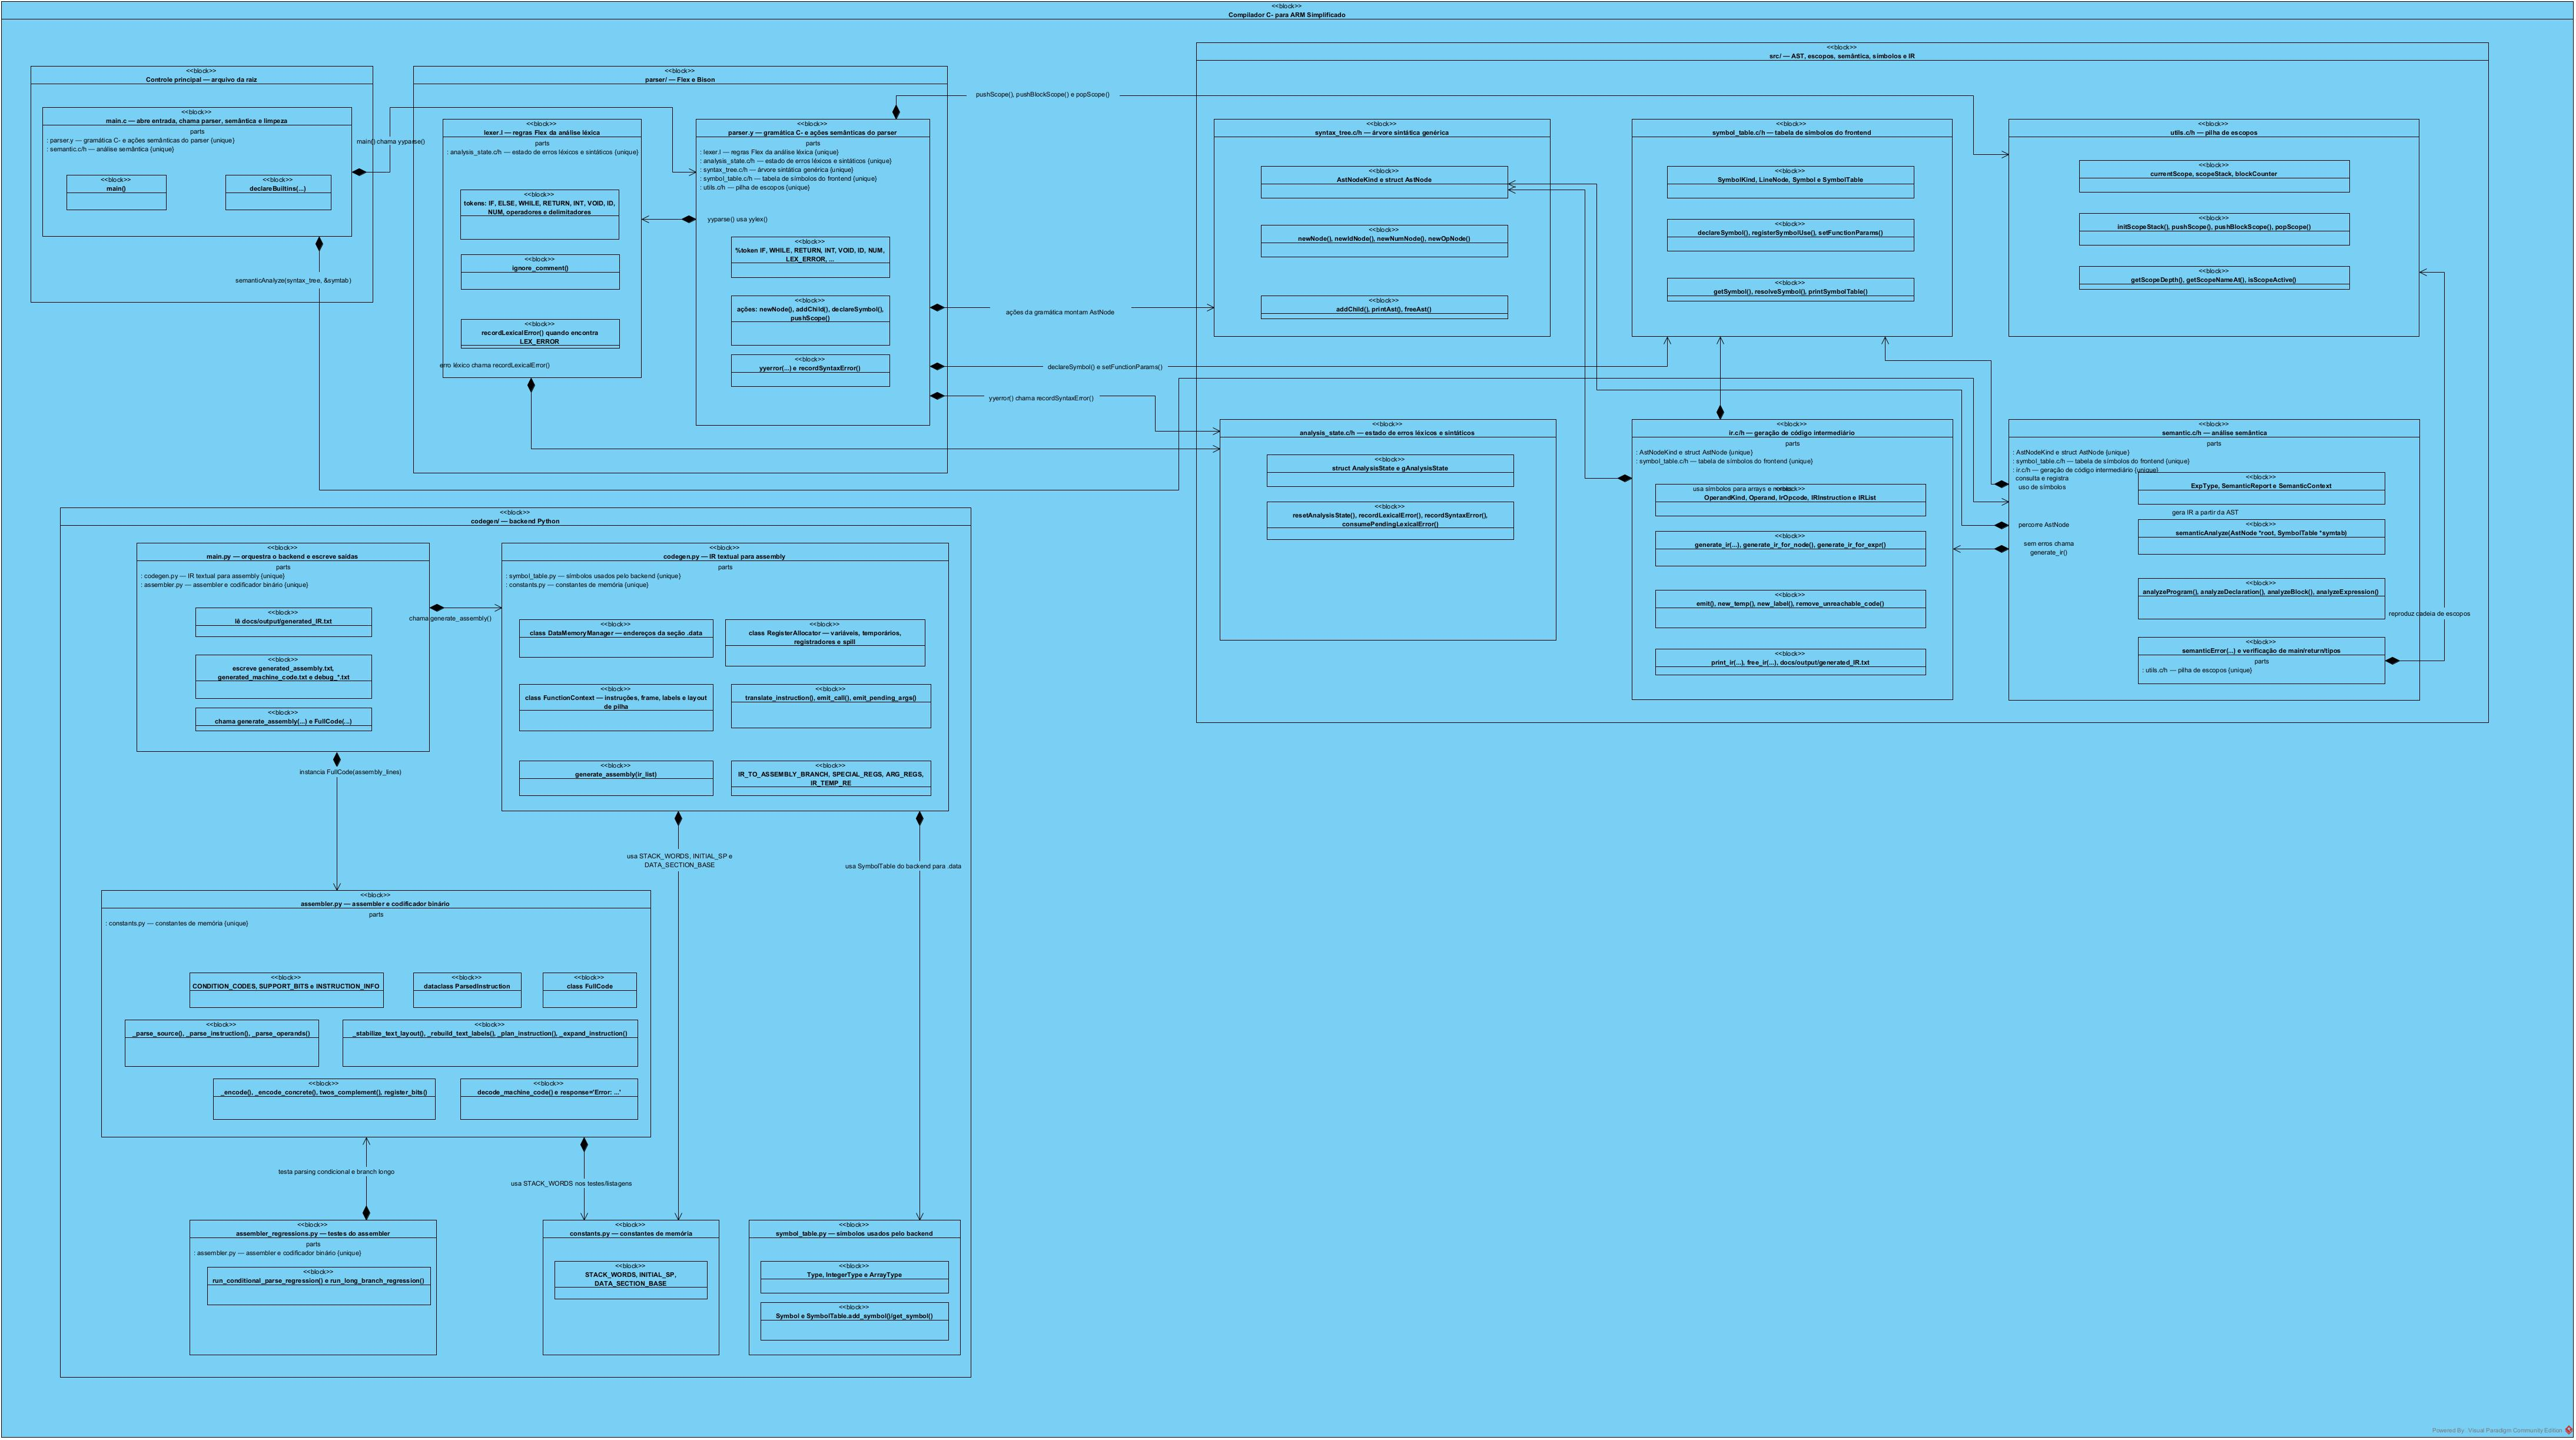
\includegraphics[width=0.96\linewidth]{figuras/hierarquia-modulos-compilador.jpg}
  \legend{Fonte: relatório de compiladores, conferido contra os arquivos atuais em \texttt{compiler/}. A figura representa dependências e responsabilidades; os artefatos sob \texttt{compiler/docs/generated/} são saídas, não fontes editáveis.}
\end{figure}
\end{landscape}

\section{Fase de análise}

O front-end é escrito em C. Flex reconhece palavras-chave, identificadores, inteiros, operadores, delimitadores e comentários; Bison aplica a gramática C- e constrói a AST. A tabela de símbolos representa funções, variáveis, vetores e escopos aninhados. A análise semântica verifica declarações, tipos, chamadas, vetores, retornos e a presença de \texttt{main}. Erros léxicos, sintáticos ou semânticos impedem a geração de IR.

\begin{table}[H]
\centering
\ABNTEXfontereduzida
\caption{Módulos da fase de análise}
\label{tab:frontend}
\begin{tabular}{|p{0.27\textwidth}|p{0.57\textwidth}|}
\hline
\textbf{Módulo} & \textbf{Responsabilidade} \\
\hline
\texttt{lexer.l} e \texttt{parser.y} & Tokens, gramática, construção inicial da AST e abertura de escopos. \\
\hline
\texttt{syntax\_tree.c/h} & Representação, impressão e liberação da AST. \\
\hline
\texttt{symbol\_table.c/h} e \texttt{utils.c/h} & Símbolos, assinaturas, usos e pilha de escopos. \\
\hline
\texttt{semantic.c/h} & Validação semântica e autorização para gerar IR. \\
\hline
\texttt{ir.c/h} & IR de três endereços, temporários, rótulos e remoção de código inalcançável. \\
\hline
\end{tabular}
\legend{Fonte: O autor, com base no código atual.}
\end{table}

\subsection{Análise léxica e controle de erros}

O scanner em \texttt{lexer.l} converte o fluxo de caracteres em tokens para palavras-chave, identificadores, números, operadores e delimitadores. Comentários são consumidos sem alcançar a gramática. Quando encontra um caractere inválido, o lexer registra o erro no estado de análise. Esse estado permite que o parser reconheça que determinada falha nasceu na etapa léxica e evita que um único caractere gere uma sequência enganosa de diagnósticos sintáticos.

\subsection{Análise sintática e AST}

A gramática em \texttt{parser.y} reconhece declarações globais, funções, parâmetros, blocos, comandos condicionais e iterativos, retornos e expressões. Suas ações semânticas criam nós da AST e registram informações necessárias à resolução posterior. A árvore elimina detalhes puramente gramaticais e preserva a estrutura relevante para tipos, controle de fluxo e geração da IR. O módulo \texttt{syntax\_tree.c} centraliza a criação, o encadeamento, a impressão diagnóstica e a liberação desses nós.

\subsection{Símbolos, escopos e análise semântica}

A pilha de escopos distingue o nível global, funções e blocos aninhados. Cada símbolo registra sua categoria, tipo, escopo de declaração, linhas de uso e, para funções, sua assinatura. A análise semântica percorre a AST para rejeitar redeclarações incompatíveis, identificadores ausentes, índices ou argumentos inválidos, usos inconsistentes de vetores, retornos incompatíveis e programas sem \texttt{main}. Ela também verifica caminhos de retorno em funções que produzem valor. Somente depois dessa etapa a IR é autorizada, preservando a regra de que um programa inválido não segue para o back-end.

\section{IR, back-end e montagem}

A IR textual é o contrato entre o front-end em C e o back-end em Python. Ela representa atribuição, endereço, load/store, declaração, aritmética, comparação, rótulos, desvios, argumentos, chamadas e retornos. O operador módulo é reduzido a divisão, multiplicação e subtração porque não existe opcode nativo correspondente.

\subsection{Representação intermediária}

O emissor de IR usa temporários e rótulos para tornar explícita a ordem de avaliação. Expressões compostas são decompostas em operações de três endereços; condicionais e laços tornam-se comparações seguidas de branches e labels; acessos a vetores distinguem obtenção de endereço e leitura ou escrita do valor. Declarações globais também aparecem na IR para que o back-end possa reservar a seção de dados. Antes da impressão, uma passagem local remove instruções inalcançáveis posteriores a desvios incondicionais ou retornos até o próximo rótulo.

O back-end calcula frames, aloca registradores, derrama temporários e emite assembly. A convenção reserva \texttt{r0} para retorno, \texttt{r1--r3} para argumentos rápidos, \texttt{r27} para expansões do montador, \texttt{r28} como link lógico, \texttt{r29} como SP, \texttt{r30} como auxiliar de spill e \texttt{r31} como FP. O montador resolve rótulos, expande imediatos e branches longos, e codifica as palavras finais.

\subsection{Frames, registradores e chamadas}

Cada função possui um contexto que associa parâmetros, locais, vetores e temporários a registradores ou posições relativas ao frame pointer. Os três primeiros argumentos usam \texttt{r1--r3}; excedentes são colocados na pilha. \texttt{r0} transporta o retorno. Quando os registradores temporários se esgotam, o alocador cria posições de \emph{spill} no frame e emite cargas ou armazenamentos por meio do auxiliar \texttt{r30}. O prólogo preserva o frame anterior e o retorno lógico, e o epílogo restaura esse estado antes de transferir o controle ao chamador.

Existe uma distinção essencial: \texttt{r28} é um registrador geral usado pela convenção do compilador, enquanto o RTL mantém também um link dedicado. O prólogo copia o retorno para \texttt{r28} quando necessário; o epílogo restaura esse valor e emite branch por registrador. Essa ponte deve permanecer documentada para evitar confundir as duas entidades.

\subsection{Montagem e codificação binária}

O montador faz mais do que substituir mnemônicos por bits. Primeiro separa \texttt{.text} e \texttt{.data}, reconhece rótulos e diretivas e calcula os endereços. Depois repete o cálculo de layout quando um imediato ou branch precisa ser expandido em mais de uma instrução. Só então codifica condição, classe, suporte, função e operandos. Esse processo iterativo é necessário porque a expansão de uma instrução altera o endereço das instruções e dos rótulos seguintes.

A \autoref{fig:codificador-binario} apresenta a decomposição funcional da última etapa. Os blocos internos são uma modelagem do comportamento de \texttt{assembler.py}, e não classes separadas no código. A figura continua válida para os campos de 32 bits e para os sete sufixos condicionais aceitos. A semântica especial de branch e retorno permanece detalhada na \autoref{tab:branch}, pois não cabe integralmente nessa visão compacta.

\begin{landscape}
\begin{figure}[p]
  \centering
  \caption{Decomposição funcional do montador e do codificador binário}
  \label{fig:codificador-binario}
  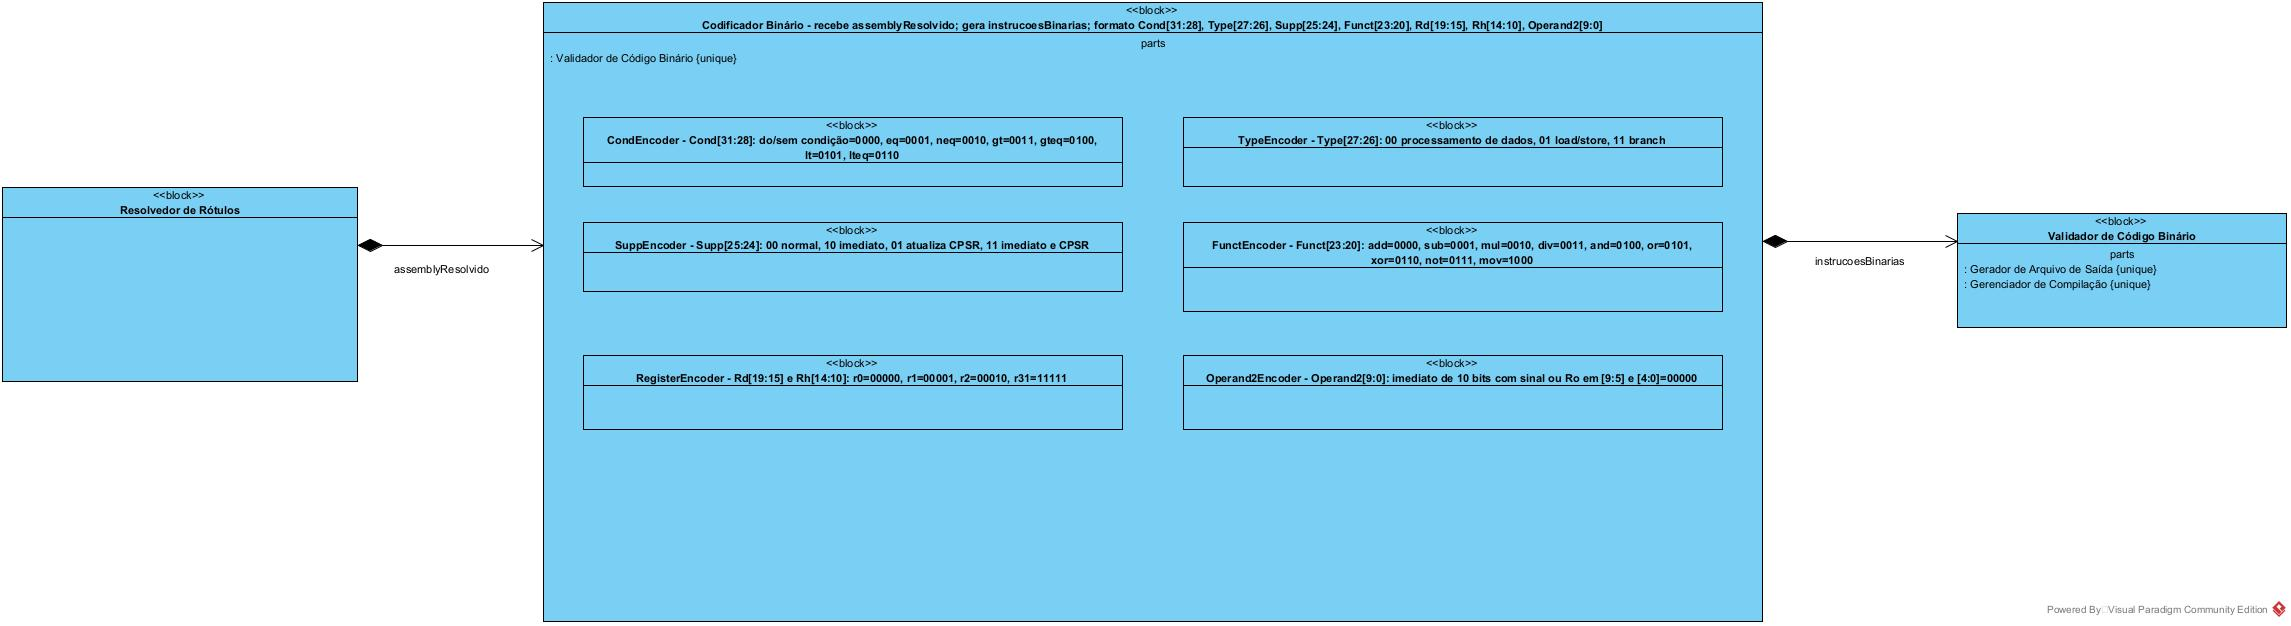
\includegraphics[width=0.96\linewidth]{figuras/codificador-binario.jpg}
  \legend{Fonte: relatório de compiladores, validado contra \texttt{compiler/codegen/assembler.py}. Os encoders mostrados são responsabilidades conceituais implementadas pelo montador.}
\end{figure}
\end{landscape}

\subsection{Exemplo validado de assembly e código de máquina}

A \autoref{fig:assembly-maquina} preserva um exemplo visual do relatório de compiladores, mas sua correspondência foi novamente verificada com o montador atual. As doze linhas exercitam imediatos, operações aritméticas, atualização de flags, branch condicional e branch incondicional. Ao executar essas mesmas linhas em \texttt{FullCode}, o montador produziu com sucesso as doze palavras mostradas, sem diferença bit a bit.

\begin{figure}[H]
  \centering
  \begin{minipage}[t]{0.42\textwidth}
    \centering
    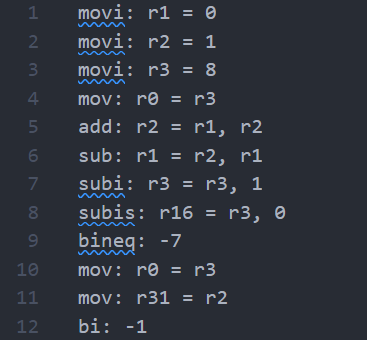
\includegraphics[width=\linewidth]{figuras/exemplo-assembly.png}
    \smallskip

    \ABNTEXfontereduzida (a) Assembly de entrada.
  \end{minipage}
  \hfill
  \begin{minipage}[t]{0.52\textwidth}
    \centering
    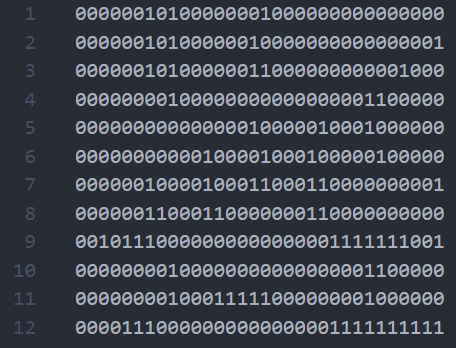
\includegraphics[width=\linewidth]{figuras/exemplo-codigo-maquina.png}
    \smallskip

    \ABNTEXfontereduzida (b) Palavras binárias produzidas.
  \end{minipage}
  \caption{Correspondência validada entre assembly e código de máquina}
  \label{fig:assembly-maquina}
  \legend{Fonte: acervo do relatório de compiladores; resultado reproduzido com \texttt{compiler/codegen/assembler.py} em 26 de setembro de 2026.}
\end{figure}

\section{Integração com ROM e modelo executável}

O gerador de MIF converte código binário em imagens de 1024 palavras de 32 bits. O simulador Python reproduz a decodificação, registradores, link, PC, flags Z/N, RAM de 64 posições, entrada e saída. Ele é evidência funcional importante, mas não prova temporização, inferência de memória, CDC, pinagem ou funcionamento físico da FPGA.

\section{Verificação reproduzida nesta consolidação}

Em 23 de setembro de 2026 foram executadas três verificações a partir da raiz do repositório. \texttt{make -C compiler test\_analysis} aprovou os casos válido, léxico, sintático, semântico, identificador não declarado e ausência de \texttt{main}; apenas a geração opcional do modelo VPP foi ignorada porque o artefato não estava presente. \texttt{python3 compiler/codegen/assembler\_regressions.py} aprovou as regressões do montador. Por fim, \texttt{make -C compiler run\_selected\_10\_diagnostics} gerou e executou os dez programas selecionados, com dez resultados esperados em dez casos.

Esses resultados sustentam a coerência funcional entre front-end, back-end, montador e modelo Python para os casos cobertos. Eles não substituem simulação do RTL, compilação Quartus, análise de timing ou teste físico em FPGA, que não foram executados nesta consolidação.

\chapter{Comparação dos relatórios e correções}
\label{cap:comparacao}

\begin{table}[H]
\centering
\ABNTEXfontereduzida
\caption{Síntese da comparação entre os relatórios e o projeto atual}
\label{tab:comparacao}
\begin{tabular}{|p{0.18\textwidth}|p{0.20\textwidth}|p{0.20\textwidth}|p{0.29\textwidth}|}
\hline
\textbf{Tema} & \textbf{Processador 2024} & \textbf{Compiladores 2025} & \textbf{Decisão atual} \\
\hline
Fundamentação & Harvard, RISC e ARM & Resume e integra ao C- & Mantida como contexto, sem alegar compatibilidade ARM. \\
\hline
ISA & Evolução histórica e sufixos & Campos de 32 bits e integração & Mantida somente na forma confirmada pelo montador e RTL. \\
\hline
Datapath & Diagrama antigo e link externo & Reutiliza o diagrama & Figura rejeitada; descrição reconstruída de \texttt{integrated.v}. \\
\hline
ROM & Inicialização textual antiga & Menciona arquivo textual em um trecho & Corrigida para \texttt{program.mif}, 1024 por 32. \\
\hline
RAM & Descrita genericamente & Afirma 64 por 32 & Registrada divergência: RTL 64 por 64, software 64 por 32. \\
\hline
Branch & Semântica anterior parcialmente histórica & Diferencia imediato, registrador e link & Atualizada para PC relativo, destino absoluto em registrador e link dedicado. \\
\hline
Compilador & Apenas assembler inicial & Pipeline C-/IR/Python completo & Conteúdo exclusivo e complementar do relatório de compiladores. \\
\hline
Testes & Waveforms e bancada de 2024 & Exemplos e simulador & Resultados antigos preservados como históricos; estado atual exige nova síntese/bancada. \\
\hline
Sistema Operacional & Não abordado & Não abordado & Declarado não implementado. \\
\hline
\end{tabular}
\legend{Fonte: O autor. A matriz expandida está em \texttt{COMPARACAO.md}.}
\end{table}

As 35 imagens disponíveis nas duas pastas do relatório de compiladores foram avaliadas individualmente. Oito foram incorporadas: placa, comparação Harvard/von Neumann, fluxo, hierarquia, codificador, waveform compatível da ULA e o par assembly/código de máquina. Permanecem rejeitadas as figuras antigas de \emph{condition field}, conjunto de instruções e caminho de dados, pois contêm divergências materiais como condição não suportada, PC por quatro, roteamento antigo da RAM ou codificação anterior. Formas de onda sem revisão ou testbench identificável também não foram tratadas como validação atual. A decisão nominal para cada arquivo está registrada em \texttt{COMPARACAO.md}.

\chapter{Lacunas para o próximo Laboratório}
\label{cap:lacunas}

\section{Lacunas do hardware e da documentação}

Antes de introduzir mecanismos de SO, a plataforma precisa de uma base mais determinística:
\begin{itemize}
  \item produzir um diagrama atual do caminho de dados a partir do RTL validado;
  \item alinhar a largura da RAM entre RTL, compilador, MIF e simulador;
  \item eliminar o alias entre a pilha de 64 palavras e a seção global iniciada no endereço 64;
  \item definir e testar o estado após reset para registradores, link, flags, RAM e saída;
  \item substituir ou justificar a distribuição de clocks derivados e criar restrições SDC;
  \item confirmar por síntese a inferência de ROM, RAM, multiplicação e divisão;
  \item criar testbenches autochecking para ISA, branches, memória, entrada e saída;
  \item executar nova compilação Quartus e nova validação em placa antes de reutilizar resultados de 2024.
\end{itemize}

\section{Lacunas de interface necessárias a um SO}

O repositório não apresenta ainda uma arquitetura de Sistema Operacional. Não foram identificados mecanismos completos de modo usuário/supervisor, exceções, tabela de vetores, instrução de retorno de interrupção, temporizador com protocolo de interrupção, chamadas de sistema, proteção de memória ou troca de contexto. O programa \texttt{10\_carga\_preempcao} é uma carga diagnóstica; seu nome não comprova preempção em hardware ou software.

Consequentemente, o próximo Lab deve começar pela especificação, e não pela documentação retrospectiva de funcionalidades inexistentes. As decisões iniciais precisam definir o modelo de execução, o contexto salvável, o evento de interrupção, o ABI de chamadas de sistema e o mapa de memória. Somente depois dessas decisões o relatório poderá afirmar a existência de processos, escalonador ou serviços de SO.

\section{Critérios mínimos para a próxima revisão}

Uma revisão futura deste documento deverá exigir evidência reproduzível para cada nova capacidade: requisito, alteração de ISA/RTL quando aplicável, produtor e consumidor atualizados, teste de software, simulação RTL, síntese e, para afirmações de bancada, execução física documentada.

\chapter{Conclusão}
\label{cap:conclusao}

Os relatórios anteriores são complementares: o primeiro explica a origem arquitetural e os módulos do processador; o segundo conecta essa máquina a um compilador C- mais amplo. A comparação com o repositório atual, porém, mostra que várias descrições visuais e operacionais ficaram desatualizadas. O principal resultado desta consolidação é separar o que permanece válido do que precisa ser novamente projetado ou comprovado.

A plataforma já possui uma cadeia funcionalmente testável de C- até código de máquina e um RTL capaz de consumir a mesma codificação. Ela ainda não possui um Sistema Operacional. Este relatório, portanto, encerra a documentação do estado inicial e fornece uma lista explícita de riscos e lacunas para que o próximo laboratório avance sobre uma base verificável.

\postextual
\bibliographystyle{abntex2-alf}
\bibliography{referencias}
\end{document}
